% \section{ARC Synthesis}
% % Operators require support for a diverse collection of policies, 
% % like service chaining, traffic engineering, and isolation. Also,
% % since failure is handled in a distributed manner, operators need 
% % support for policies which specify resilience properties and behavior
% % of traffic under failure scenarios. 
% % Earlier 
% % work in this area has focused on finding ideal OSPF weights for 
% % traffic engineering~\cite{te-ospf}, but such approaches are 
% % inherently tied with the policies supported, and are not extensible 
% % to other policies easily. 

% In our preliminary approach to ARC synthesis, 
% we tried to specify policies using SMT theories like propositional logic and 
% linear rational arithmetic and 
% use off-the-shelf SMT solvers~\cite{z3} 
% to synthesize the ARC. However, current SMT solvers are incapable of 
% scaling to even small-sized topologies and number of policies, majorly
% due to the fact the paths in the network are based on the weights in a 
% complicated manner (shortest-path) which increases the complexity of the
% encoding in SMT. Synthesizing resilient control planes with this 
% approach is intractable with current state-of-art SMT solvers.

% While the ARC synthesis from data planes can enforce 
% policies by the distributed control plane, it does not
% encapsulate resilience properties of the control plane. 
% To accomodate resilience properties in the ARC synthesis,
% we envision two different mechanisms: concrete
% backup paths and path-level policies under failure scenarios. 
% We discuss this in \secref{sec:resilience}. \kausik{Could expand more,
% write after resilience section is complete}

\section{Pure ARC Synthesis}
We first describe the synthesis of a type of ARC 
called {\em pure} ARC which
only forwards packet bases on shortest-paths and does 
not support additional mechanisms like filtering etc. 
Thus, 
the ARC is a directed graph comprising of switches as 
vertices and weighted edges corresponding to all links in the
topology (no link is disabled by any mechanism). 
This is 
a ideal control plane because it is able to enforce the data plane
with carefully engineered edge weights and no links are disabled. 
For a given network data plane, the synthesis of 
the pure ARC reduces to a
variation of the {\em inverse shortest path} problem, an almost 
unexplored algorithmic problem. 

Formally, this variation of inverse shortest path problem 
has as input: (1) a directed graph $T = (S, L)$ (the network topology), 
(2) a set of endpoints $\Gamma$, and 
(3) a set of paths $P$
such that for each $(s,t) \in \Gamma, \exists p \in P$ such
that the path $p$ is from $s$ to $t$. 
The problem is to find weights for the edges $L$ such that 
for each $(s,t) \in \Gamma$, every lowest weighted path 
in the graph 
from $s$ to $t$ is in set $P$. 

From the paths in the data plane, 
we extract the forwarding
DAG (directed acyclic graph) for each destination
as the sink (as the forwarding is destination-based). 
We define $\Omega$ for the 
set of destinations, and $\Delta$ for  
the set of destination DAGs. 
Given $\Omega$ and $\Delta$, we generate a set of linear equations
to find the requisite edge weights of a pure ARC. 
For this, we define $E(sw_1, sw_2)$ as
the edge weight variable for link $sw_1 \rightarrow sw_2$. 
For a path connecting two switches 
$s \rightarrow^+ t$ in a DAG, 
to enforce that the path will be the shortest, we need equations
which ensure the sum of edge weights of the path is strictly smaller than
the weight of all other paths from $s$ to $t$. However, this can incur
an exponential blow-up in number of equations. Instead, we use distances 
to reduce the number of equations to a polynomial order. 

\minisection{Distance Equations}
$D(s,t)$ denotes the absolute shortest distance from $s$ to $t$. 
Trivially, $D(s,s) = 0$. For a path $s \rightarrow^+ t$ ($len \geq 1$),
the shortest distance from $s$ to $t$ is the smallest of the distances
of the paths traversed through the neighbours of $s$ to $t$. Therefore, the
following set of equations enforce the semantics of distances; 
here $s \rightarrow sw$ denotes that $sw$ is a neighbour
of $s$, and $sw \rightarrow^* t$ denotes that the path from $sw$ to $t$ contains
zero or more edges.
\begin{multline} \label{eq:dist}
\forall s, t, sw. (s \rightarrow sw \rightarrow^* t).\\
D(s, t) \leq E(s, sw) + D(sw, t)
\end{multline}
These equations ensure that $D(s,t)$ is not greater than 
the actual shortest distance from $s$ to $t$.

\minisection{Destination DAG Equations}
For each destination DAG, we add equations to ensure the 
edge weights are set such that a shortest-path forwarding in the ARC 
follows the same path or paths specified in the DAG. If a path
is the shortest path between its endpoints, then every 
subpath of the path has to be the shortest between its endpoints
as well. 
\begin{figure}[h!] 
	\centering
	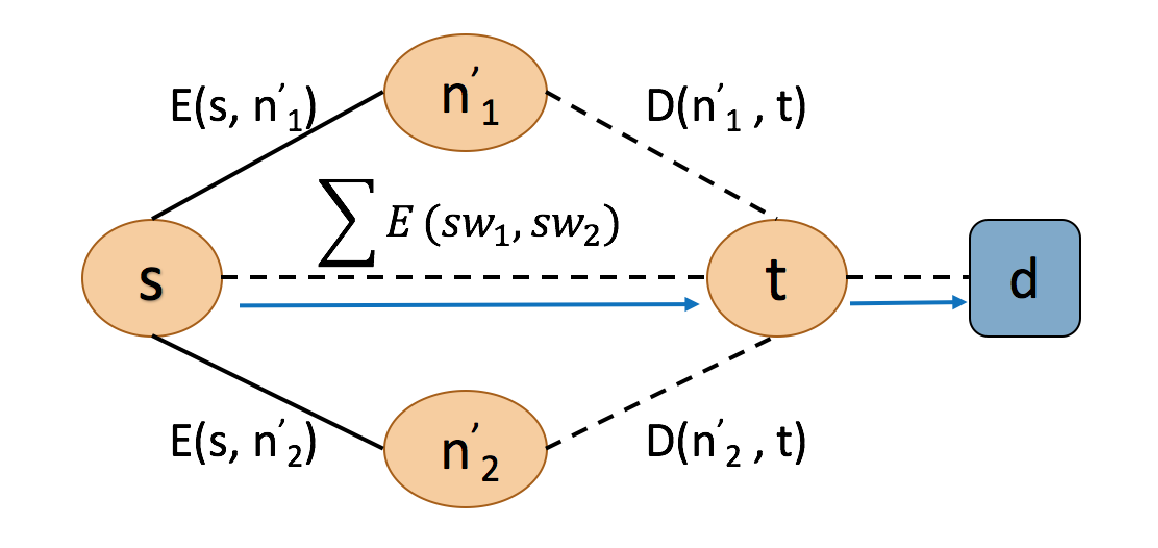
\includegraphics[width=0.8\columnwidth]{figures/distanceEquation.eps}
	\caption{Distance equation} \label{fig:disteq}
\end{figure}
Consider a DAG $\xi_d$ for destination $d$. We define two neighbour
functions: $N(s)$ denotes the set of neighbours of switch $s$ 
in the directed graph, and $N(s, \xi_d)$ denote the set of
neighbours of switch $s$ in the destination DAG. 
Since, each subpath of $\xi_d$ is the shortest path,
we need to ensure that all other
paths are not shorter or equal to these paths.  
We express the weight of the  
path in the DAG by the sum of weights of 
edges along the path. 
Thus, we add the following equations to ensure the
shortest path property (\Cref{fig:disteq} illustrates 
an example).
\begin{multline} \label{eq:uniq}
		\forall d \in \Omega. \forall s, t \in \xi_d. (s \rightarrow^+ t).\\ 
		\forall n'. (n' \in N(s) \wedge n' \not\in N(s, \xi_d)). \\
		\sum_{\mathclap{\substack{(sw_1, sw_2) \in (s \rightarrow^+ t)}}} 
		E(sw_1, sw_2) < E(s, n') + D(n', t)
\end{multline}
By using distance for the path $n' \rightarrow t$, we 
are able to find lower bounds to the weight of the non-DAG 
paths from $s$ to $t$,
thus avoiding the blow-up of enumerating all paths from $s$
to $t$. 

% If the path $n' \rightarrow^* t$ 
% is not in any DAG completely, then
% $D(n',t)$ can be smaller than the actual shortest distance by the
% semantics of \Cref{eq:dist} (as
% $D(n',t)$ is not equal to any quantity by \Cref{eq:shortest}).
% However, since $D(n',t)$ is on the RHS of the equations in \Cref{eq:uniq},
% the equations will ensure that the path $s\rightarrow n \rightarrow^* t$
% has strictly greater weight than the path of the DAG.

%TODO: Add some figures